\section{Provided Hardware}\label{sec:hardware}
%The quadcopter has been provided by Aalborg university and professor Henrik Shjøiler\fixme{add danish letters}. This chapter has the purpose of describing the hardware. 
%The hardware is tested and the results of these test will be presented. 
The provided hardware is described in this section. This is to give an overview of the initial configuration of the system, as it influences the design leading to the final prototype. The provided quadcopter including additional hardware is seen in \autoref{fig:systemBase}.
%
\begin{figure}[H]
  \centering
  \includegraphics[width=.7\linewidth]{figures/SDPhotowithNumbers.pdf}
  \caption{The quadcopter with the given hardware.}
  \label{fig:systemBase}
\end{figure}
%
The provided quadcopter framework measures 45 cm from rotor to rotor and is an X-shaped symmetric quadcopter, with a height of 7.5 cm. With the provided and selected hardware the total mass of the quadcopter is 996 g.

\subsection{Motors}
The quadcopter is equipped with four brushless DC outrunner motors named Turnigy Multistar. Contrary to brushed DC motors these do not rely on a brush which is susceptible to mechanical wear. Outrunner motors have their magnets (rotor) in the outer shell. The rotor spins around the fixed coils that form the stator. Outrunner motors generally have more space for magnets compared to inrunner motors, which is why outrunner motors typically have more poles, and thus, are able to produce more torque for the same physical dimensions. 

The motor has a motor velocity constant, $k_v$, of \SI{935}{RPM\ V^{-1}}, has 14 poles and a maximum current of \SI{15}{A} \cite{HkingPropeller}.

The motor used is shown in \autoref{fig:Motor}.
\begin{figure}[H]
	\centering
	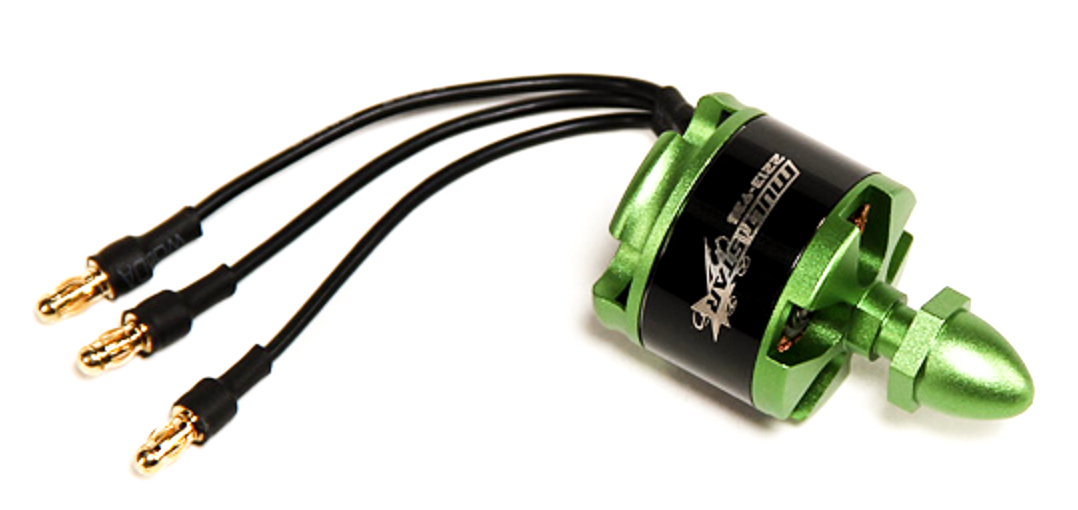
\includegraphics[scale=0.5]{figures/motorphoto.png}
	\caption{One of the four motors mounted on the quadcopter.\cite{HkingPropeller}}
	\label{fig:Motor}
\end{figure} 

\subsection{Propellers}
The propellers have a length of \SI{25.4}{cm} and a pitch of \SI{11.43}{cm}. The pitch is the distance traveled by a propeller after one complete rotation. For this to be true the propeller must turn inside a solid surface, the traveled distance is less if it rotates inside a liquid or gas \cite{EReyes}. A higher pitch creates more turbulence and make the quadcopter less steady when flying \cite{oscarliang}.

A longer propeller has an increase in the quadcopter's speed. The acceleration of a small propeller is greater than that of a larger propeller. Thus it is easier to change the moment of inertia if utilizing a small propeller compared to a larger one. \cite{oscarliang}

In this case the given propellers are suitable for the utilized quadcopter, as they have been utilized in multiple cases before. 

A picture of the utilized propellers can be seen in \autoref{fig:Propeller}.

\begin{figure}[H]
	\centering
	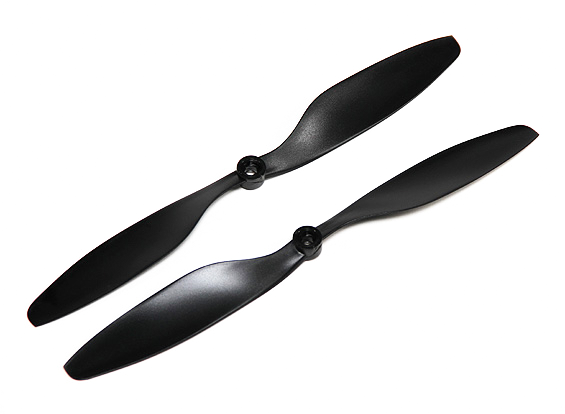
\includegraphics[scale=0.6]{figures/propellerphoto.png}
	\caption{Two of the four propellers mounted on the quadcopter's motors.\cite{HkingPropeller}}
	\label{fig:Propeller}
\end{figure}

%The relationship between PWM signal to the motor controllers and the velocity of the propeller can be seen in Figure ZZ. \fxnote{pull diagram from measurement report}

%It has been observed during tests, that the motor runs faster as it's temperature increases. This is not expected due to the increased resistance, that occurs when the coils within the motor are heated. Therefore the relationship between PWM signal and velocity is not representative for all cases. It is however deemed reasonable to neglect this variance and presume a relationship as it is derived in the measurement report, see Appendix YY.

\subsection{Motor Controllers}\label{subsec:ESC}
The quadcopter comes with four electronic speed controllers, ESCs, one for each motor. The ESCs produce an \SI{8}{kHz} PWM, are rated for a 2-4 cell Li-Po battery and can handle a constant current of up to \SI{30}{A}. The ESCs have also a \SI{5.5}{V}, \SI{4}{A} output for powering e.g. a controller board. The battery level is only measured at start up, which can be problematic, as the provided power will decrease as the battery level drops over time. \cite{HKing}

%
\begin{figure}[H]
	\centering
	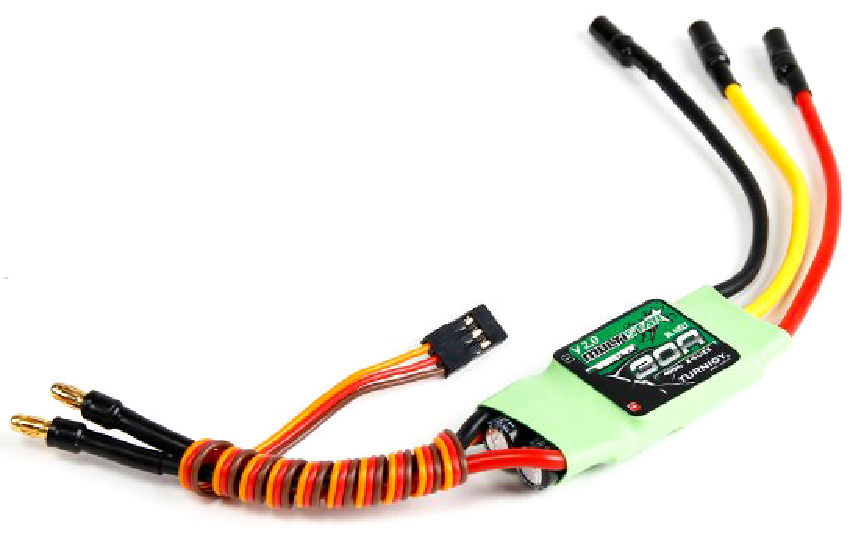
\includegraphics[scale=0.6]{figures/MotorControllerPhoto.pdf}
	\caption{One of the four Electronic Speed Controllers mounted on the quadcopter.\cite{HKing}}
	\label{fig:esc}
\end{figure}
%
\subsection{Battery}
The battery available for the prototype, is a Turnigy battery. It has a capacity of \SI{2200}{mAh}, a voltage of \SI{11.1}{V} and a discharge rate of 20-30 C.\cite{HKingBattery}

\begin{figure}[H]
	\centering
	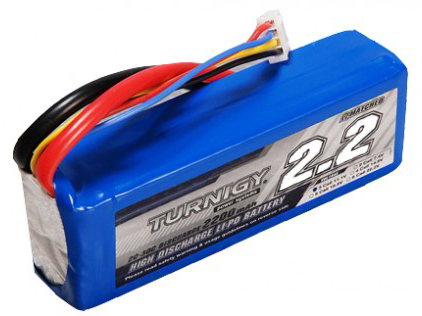
\includegraphics[scale=0.5]{figures/BatteryPicturephoto}
	\caption{The battery mounted on the quadcopter.\cite{HKingBatterypicture}}
	\label{fig:battery}
\end{figure}
%
%The battery level drops over time, with a significance that can not be neglected as it may have great impact on the output of the motor and therefore on the lift of the propeller. It is possible to measure the battery level while operating the quadrotor. By taking into account the battery level in the test of the PWM signal to velocity, it is possible to obtain a quadcopter having constant lift force, if this is requested. With this information and knowledge of the relationship between voltage and RPM, see \autoref{app:VoltageLevelTest}, it is possible to account for the battery level in the control realization and thereby rectify the problem.

\section{Selected hardware}
The provided quadcopter is not capable of flying as it is. Therefore additional hardware must be implemented. This includes sensors, as the quadcopter will otherwise not be able to navigate. A processor, as a computation device is needed to handle the communication and the control algorithms. And lastly a wireless module, as communication with the quadcopter is required. The chosen sensor solution is now presented.

\subsection{Sensor}
It is possible to implement on board sensors or use a real time attitude and position data capturing system such as Vicon, which is available at Aalborg University in a room of the dimensions: 5.85 m $\times$ 5.72 m $\times$ 3.72 m .
As the focus of this project is to design and implement a control system in a distributed network, it is chosen to use the Vicon system. This challenges the control system by introducing network delays and packet loss. As this project develops a prototype, it is not essential that the quadcopter can operate outside of the Vicon system.

The Vicon system provides real-time position and attitude captured with nine infrared cameras.
%An example is found in Aalborg University as seen in \figref{ViconRoom}. 
%
%\begin{figure}[H]
%	\centering
%	\includegraphics[scale=0.5]{figures/ViconRoom}
%	\caption{Aalborg University's Vicon room.}
%	\label{ViconRoom}
%\end{figure}

To use this system, reflective markers are attached to the tracked object. The Vicon system streams the position of the markers and the position and attitude of the object at 100 Hz for a computer to read them\cite{ViconDataSTream}. The data can be received by using an SDK (software development kit) plug-in for MATLAB. In this way, data can be received by MATLAB, making it possible to directly perform calculations, which makes it easier to obtain variable derivatives.

The user interface of the Vicon system is shown in \autoref{fig:ViconTracker} and an illustration of the Vicon system setup is seen in \autoref{fig:Vicontotalsystem}. 
%
\begin{figure}[H]
	\centering
	\captionbox
	{
		User interface of the Vicon System, the Vicon Tracker. An object has been created from the markers placed on the quadcopter..
		\label{fig:ViconTracker}
	}
	{
	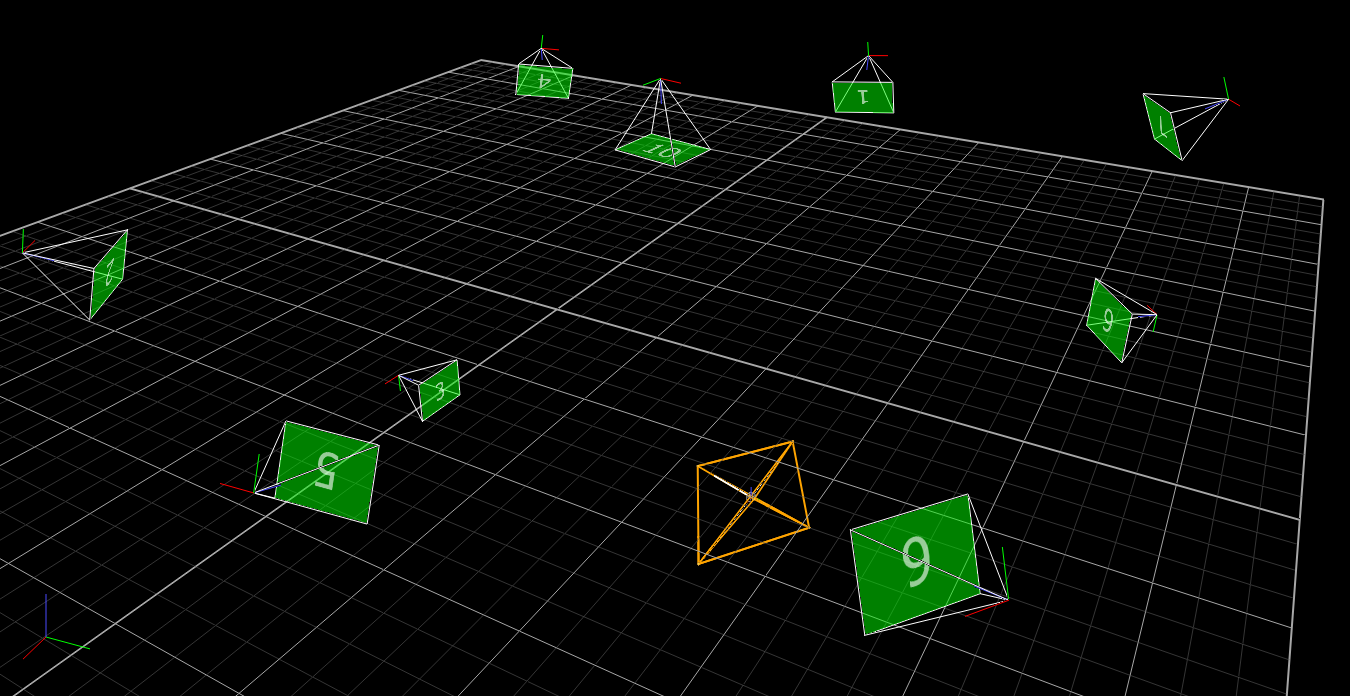
\includegraphics[width=.5\textwidth]{figures/ViconTracker3}
	}
  \hspace{5pt}
  \captionbox
  {
  	An illustration showing the Vicon system's cameras sensing the quadcopter and the computer used to get the data.
  	\label{fig:Vicontotalsystem}
  }
  {
  	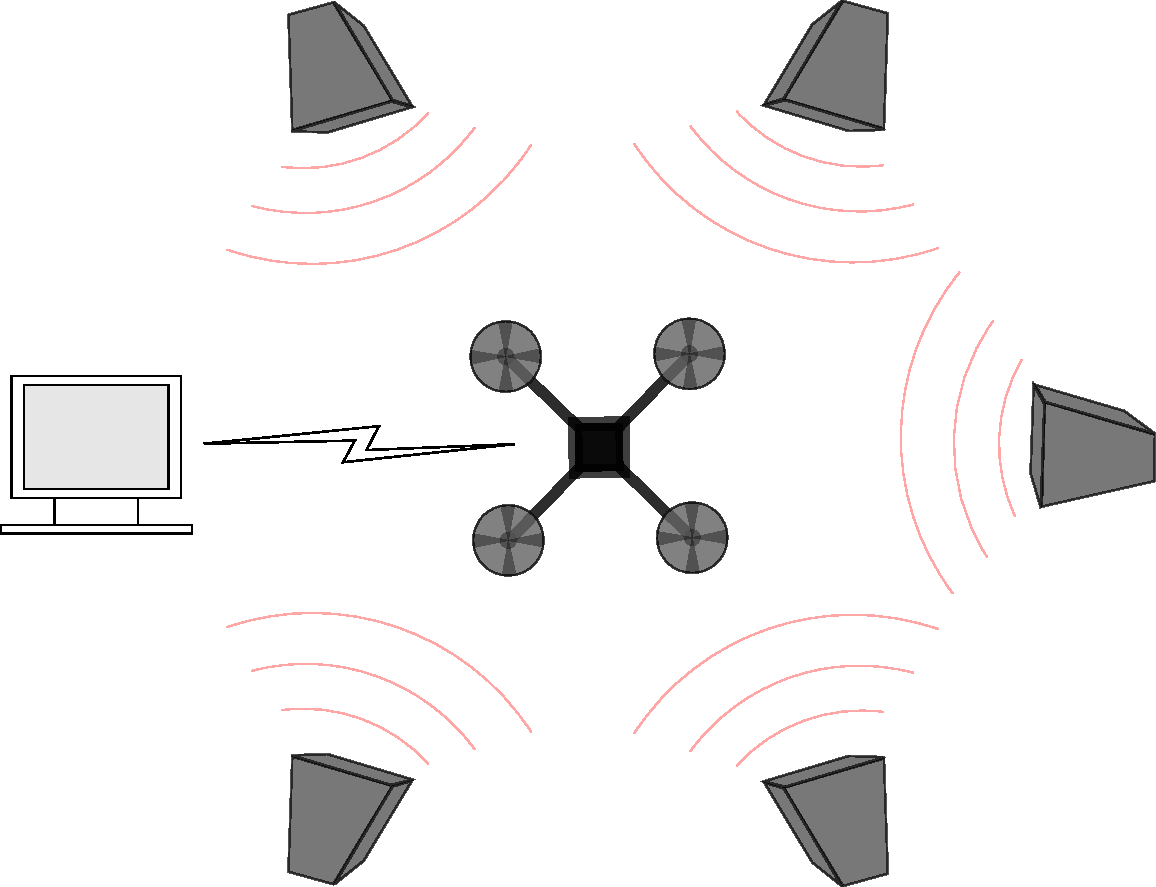
\includegraphics[width=.40\textwidth]{figures/system.pdf}
  }
\end{figure}
The software is called Vicon Tracker and it allows the creation of objects by grouping markers present in the room. It also allows to change the center of gravity of the created objects and rotate the inertial and body reference frames to any desired orientation.

\subsection{Processor}
As the computer on the ground only handles the Vicon sensor data and the communication of this data, the processor of the quadcopter must be capable of handling the processing of the control while also receiving the attitude and position of the quadcopter.
The implementation of the controllers is done in a microprocessor from Atmel, ATmega2560, mounted on the ArduinoMEGA development board, as seen in \autoref{fig:ATmega}. This processor has up to 16 PWM output channels, two 8-bit timers and four 16-bit timers, four USART modules, 8 kB of internal memory and a processing speed of 16M IPS. These capabilities are presumed to be sufficient for the control implementation on the quadcopter.\cite{ATmega2560}

%The use of the development board makes the use of the wireless modules easier as an arduino shield can be directly plugged in. Furthermore, it allows a faster set up of the microcontroller as all required hardware (oscillatior, power supply, etc.) is already present in the board. 
\begin{figure}[H]
	\centering
	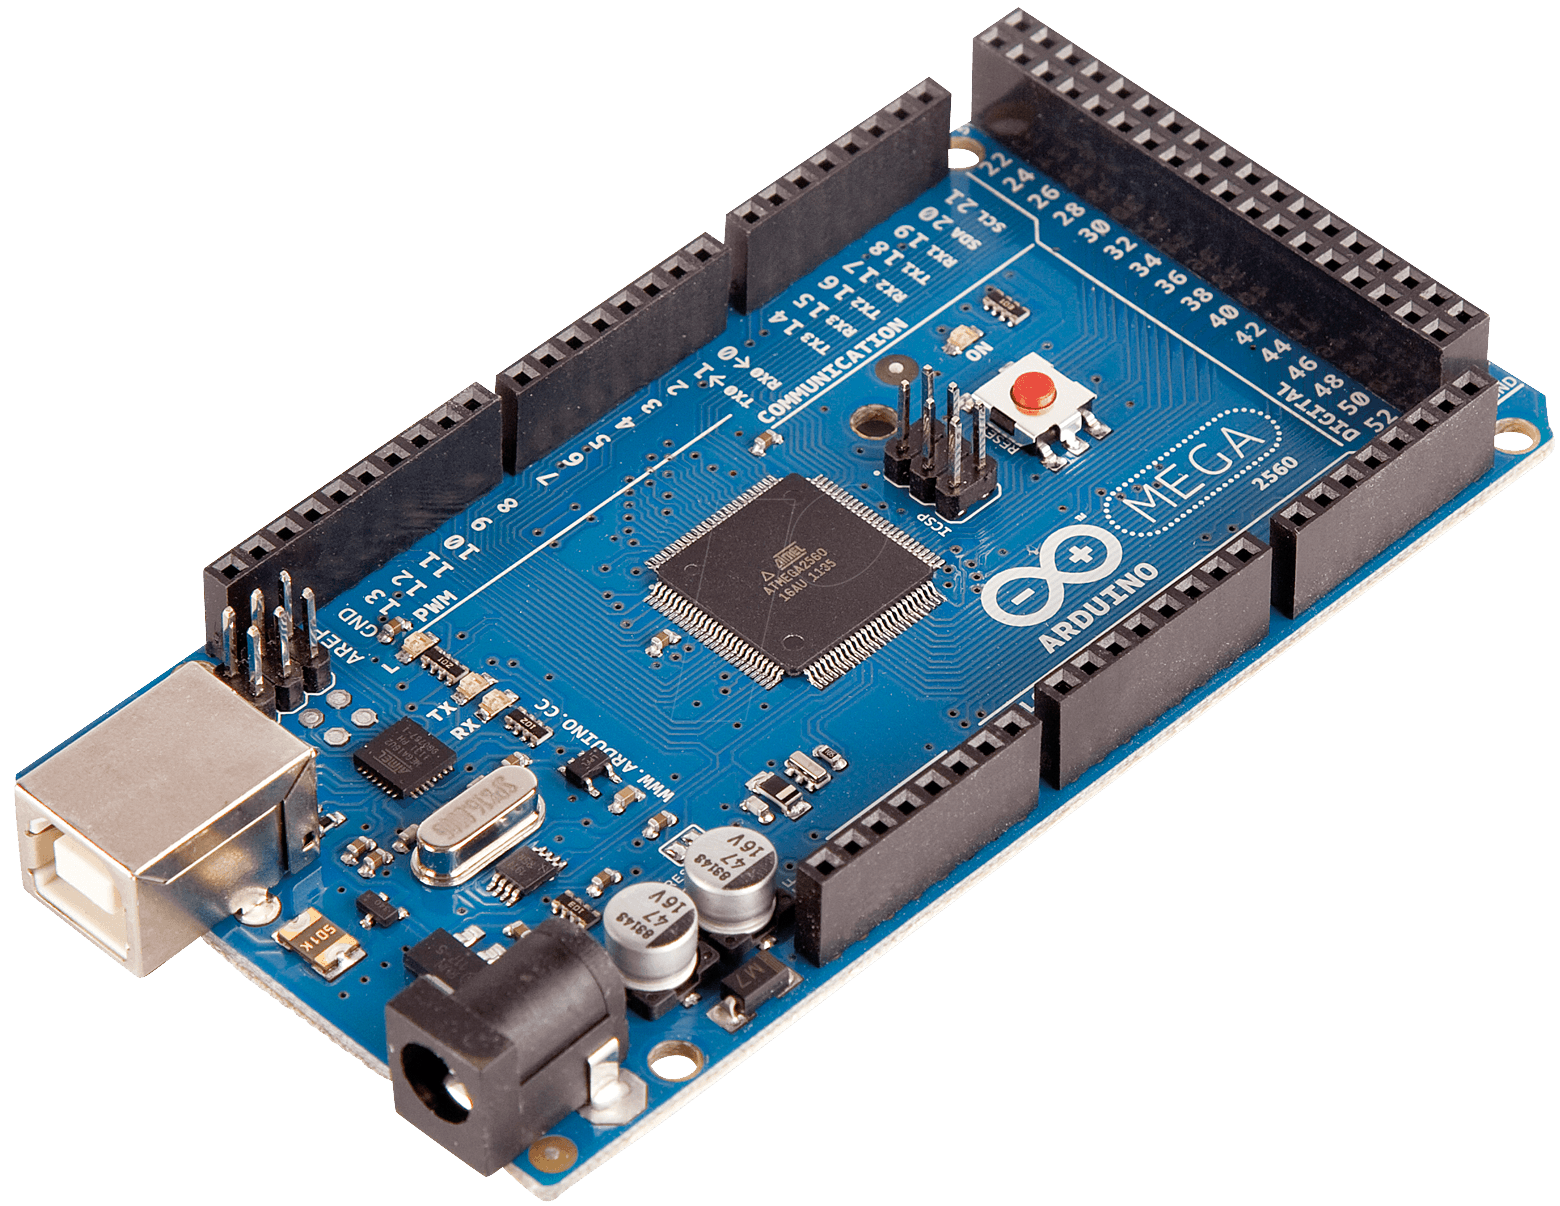
\includegraphics[scale=0.12]{figures/ARDUINO_MEGA}
	\caption{AtMega2560 mounted in the ArduinoMEGA development board.\cite{ArduinoMegaImage}}
	\label{fig:ATmega}
\end{figure}
%
\subsection{Wireless Modules}
The wireless modules used to communicate with the quadcopter are called XBee, see \autoref{fig:XBEE}. These modules need a supply voltage between \SI{2.8}{V} and \SI{3.4}{V}, which fits well with the \SI{3.3}{V} supply provided by the Arduino board\cite{XBee}.
%
\begin{figure}[H]
  \centering
  \includegraphics[scale=0.25]{figures/XBEE}
  \caption{XBee wireless modules.\cite{XBeeImage}}
  \label{fig:XBEE}
\end{figure}
%
The XBee modules communicate at a frequency of \SI{2.4}{GHz} and has a range of up to \SI{30}{m} in indoor environments and a line-of-sight range of up to \SI{90}{m}. The modules transmit with an RF data rate of \SI{250}{Kbps} and are capable of communicating with a serial interface data rate of from \SI{1200}{bps} up to \SI{250}{Kbps}. The XBee modules take care of all communication layers except the transport layer protocol. The protocol used by the XBee modules is called ZigBee, which follows the IEEE $802.15.4$ standard.\cite{XBee}
%
\begin{figure}[H]
  \centering
  \captionbox
  {
    UartSBee v4.0 USB to\\ serial adapter module. \cite{UartSBee}
    \label{fig:UartSBee}
  }
  {
    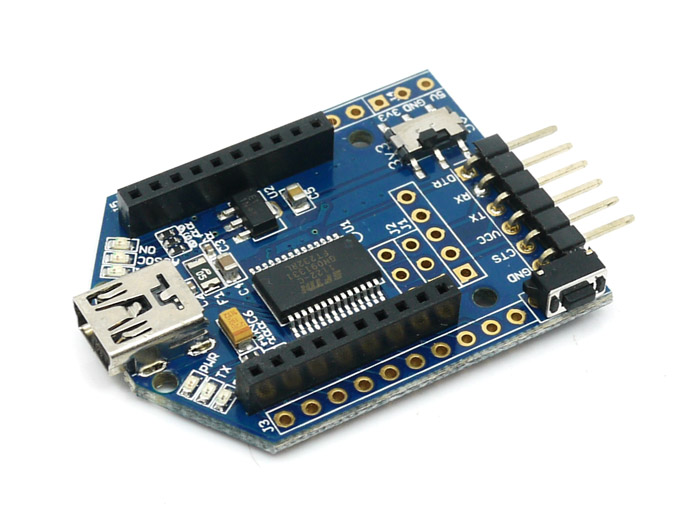
\includegraphics[width=.37\textwidth]{figures/UartSBee}
  }
  \hspace{5pt}
  \captionbox
  {
    XBee Shield. \cite{XBeeShield}
    \label{fig:XbeeShield}
  }
  {
    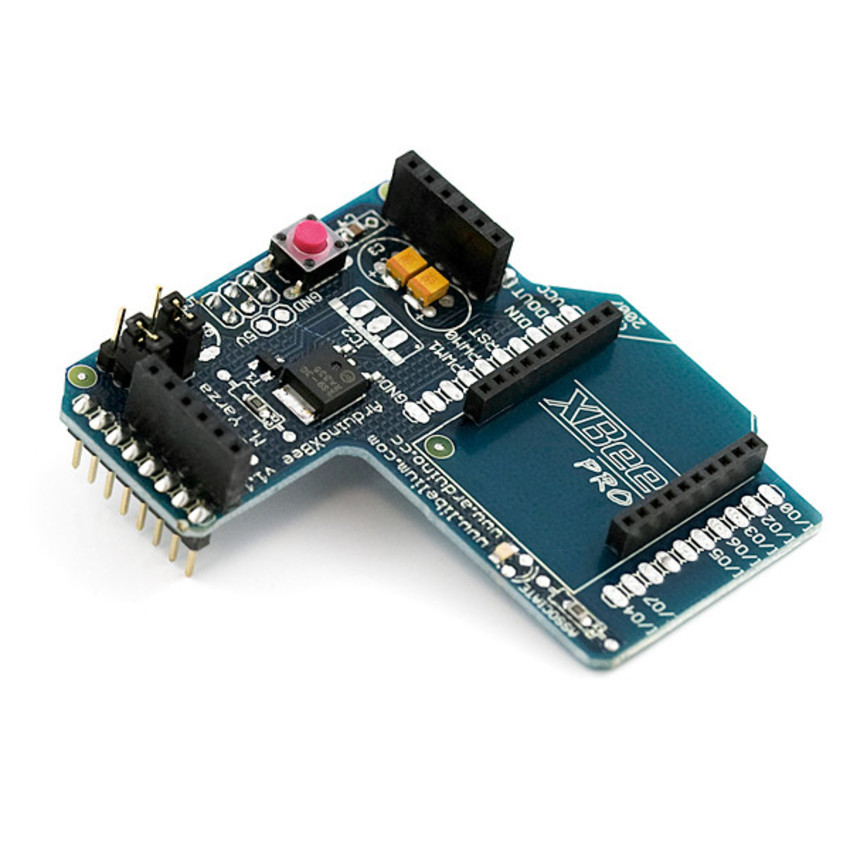
\includegraphics[width=.37\textwidth]{figures/XbeeShield}
  }
\end{figure}
%
In order to use these modules, the packet has to be sent through the serial port of the computer to the XBee, through RF to the other XBee and back through serial pins to the microcontroller. In order to interface with the XBee modules, serial connections are required on both ends, and the XBee modules must be powered. For the computer a USB to serial adapter board, called UartSBee v4.0, is used, this module also powers the XBee through the USB \cite{UartSBeeSch}. The microcontroller uses an XBee shield to connect the power and serial pins of the Arduino\cite{XbeeShieldSch}.